% SIGMOD/PACMMOD-style paper draft.
% For double-anonymous submission, change the documentclass to include
% anonymous,review and remove/replace author metadata as required by SIGMOD.
\documentclass[sigconf,screen]{acmart}

\AtBeginDocument{%
  \providecommand\BibTeX{{Bib\TeX}}}

\setcopyright{none}
\copyrightyear{2026}
\acmYear{2026}
\acmDOI{}
\acmISBN{}
\acmConference[SIGMOD 2026]{ACM SIGMOD Conference on Management of Data}{May 31--June 5, 2026}{TBD}
\settopmatter{printacmref=false}

\usepackage{amsmath}
\usepackage{amsthm}
\usepackage{algorithm}
\usepackage{algpseudocode}
\usepackage{booktabs}
\usepackage{graphicx}
\usepackage{multirow}
\usepackage{xspace}

\newtheorem{theorem}{Theorem}

\newcommand{\us}{\(\mu\)s\xspace}
\newcommand{\ops}{ops/s\xspace}
\newcommand{\sys}{Adaptive Fanout B-Tree\xspace}

\begin{document}

\title{The Cost of Adaptivity: Online Fanout Selection in Cache-Conscious B-Trees}

\author{Ranjan V}
\orcid{0009-0001-2345-6789}
\email{ranjan.v@example.edu}
\affiliation{%
  \institution{Vellore Institute of Technology, AP}
  \department{School of Computer Science and Engineering}
  \city{Amaravati}
  \state{Andhra Pradesh}
  \country{India}
}

\author{Ajit Jubilson E}
\orcid{0009-0002-3456-7890}
\email{ajit.jubilson@example.edu}
\affiliation{%
  \institution{Vellore Institute of Technology, AP}
  \department{School of Computer Science and Engineering}
  \city{Amaravati}
  \state{Andhra Pradesh}
  \country{India}
}

\begin{abstract}
B-trees traditionally use a fixed fanout chosen when the index is created.
Recent cache-conscious and workload-aware design intuitions suggest a more
adaptive alternative: hot regions should use small fanout to improve cache
locality, while cold regions should use larger fanout to reduce tree height.
This paper asks whether such online fanout adaptation can outperform strong
static B-tree baselines on realistic in-memory workloads.

We implement multiple adaptive B-tree variants, including global adaptive
trees with reinforcement-learning, regression, and ant-colony-inspired
policies, and a segmented adaptive B-tree whose key ranges adapt independently.
We compare them against static fanouts, segmented static trees, and oracle
baselines that know workload phase boundaries.  Our finding is negative but
diagnostic: the oracle benefit of changing fanout is usually smaller than the
measured cost of monitoring, records metadata, policy checks, and rebuilds.
We evaluate a production-grade baseline scaling to 31.7M ops/sec and
demonstrate that under rapidly shifting temporal skew, segmented adaptation
achieves only \(0.63\times\) the throughput of a static baseline, confirming
our theoretical break-even model.
On five-trial YCSB experiments, segmented adaptation reaches only
\(0.81\times\), \(0.74\times\), and \(0.67\times\) of static fanout-64
throughput on workloads A, B, and C.  On a shifting hot-region workload,
oracle fanout selection reaches \(1.08\times\), but segmented adaptation
reaches \(0.92\times\).  On a Wikipedia pageview trace, static fanout
selection has almost no headroom, while adaptation reaches \(0.81\times\).

We derive a simple break-even model showing that adaptation can win only when
per-operation fanout benefit exceeds monitoring, metadata, and policy cost,
plus amortized rebuild cost.  The model explains our measurements and provides
a practical diagnostic framework for future adaptive index designs.
\end{abstract}

\begin{CCSXML}
<ccs2012>
 <concept>
  <concept_id>10002951.10002952.10003190.10003192</concept_id>
  <concept_desc>Information systems~Database performance evaluation</concept_desc>
  <concept_significance>500</concept_significance>
 </concept>
 <concept>
  <concept_id>10002951.10002952.10003190.10003194</concept_id>
  <concept_desc>Information systems~Database query processing</concept_desc>
  <concept_significance>300</concept_significance>
 </concept>
 <concept>
  <concept_id>10002951.10002952.10003190.10003195</concept_id>
  <concept_desc>Information systems~Data access methods</concept_desc>
  <concept_significance>500</concept_significance>
 </concept>
</ccs2012>
\end{CCSXML}

\ccsdesc[500]{Information systems~Database performance evaluation}
\ccsdesc[500]{Information systems~Data access methods}
\ccsdesc[300]{Information systems~Database query processing}

\keywords{B-trees, cache-conscious indexing, adaptive indexing, negative results, workload-aware systems}

\maketitle

\section{Introduction}

B-trees remain one of the most important index structures in data management
systems \cite{bayer1972organization,comer1979ubiquitous,graefe2011modern}.
Despite decades of engineering, an apparently simple parameter still matters:
fanout.  A larger fanout decreases tree height and reduces pointer chasing,
but it also creates larger nodes that span more cache lines and increase
in-node search cost.  A smaller fanout improves locality inside hot nodes but
requires more levels.  Cache-conscious indexes exploit this trade-off
\cite{rao1999cache,rao2000making,chen2001fractal}, yet most systems choose a
single fanout for an entire index.

The adaptive fanout hypothesis is appealing.  Real workloads are skewed
\cite{zipf1949human,cooper2010benchmarking}: a small fraction of keys often
receives most accesses.  If an index could identify hot regions, it could use
small fanout there to keep nodes compact; if it could identify cold regions, it
could use large fanout there to reduce height.  The resulting tree would be
neither globally small nor globally large, but locally matched to access
patterns.  This paper tests that hypothesis.

We began with the optimistic expectation that online adaptation would improve
skewed workloads.  Instead, the measurements show a different and, we argue,
more useful result.  There is measurable oracle headroom: phase-aware fanout
choices can improve shifting workloads by roughly \(8\%\).  However, online
adaptation must pay for monitoring, metadata maintenance, policy evaluation,
and rebuilding.  In our in-memory setting these costs are comparable to, and
often larger than, the entire fanout-selection benefit.  The result is that the
adaptive variants lose even when the oracle proves that a better fanout exists.

We also stress-test the implementation as a systems artifact.  The baseline
B+ tree uses optimistic lock coupling and scales from 3.14M ops/sec on one
thread to 31.7M ops/sec on 32 worker threads for a one-million-key,
ten-million-operation workload.  Under rapidly shifting temporal skew, where
the hot 20\% of keys moves every one million operations, segmented adaptation
achieves only \(0.63\times\) the throughput of the static baseline.  This
front-page result is the empirical counterpart of our break-even model:
adaptation can be amortized only when fanout benefit exceeds monitoring,
metadata, policy, and restructuring costs.

This paper makes five contributions.

\begin{enumerate}
  \item We implement production-style adaptive B-tree variants, including
  reinforcement-learning, regression, ant-colony-inspired, and segmented
  adaptive policies.
  \item We add oracle baselines that quantify the best possible benefit from
  fanout changes under known phase boundaries.
  \item We isolate overheads through a clean ablation: static B-tree, static
  regions, monitoring, records metadata, monitor-plus-records, and full
  adaptation.
  \item We report a negative result on YCSB-style workloads, shifting hot
  regions, and a Wikipedia pageview trace.
  \item We derive a break-even condition that explains when online fanout
  adaptation can and cannot win.
\end{enumerate}

Our position is not that fanout is irrelevant.  Static fanout choices still
matter, and static regional indexes sometimes improve throughput.  The
diagnostic lesson is narrower: fine-grained online fanout adaptation for
in-memory B-trees must be evaluated against oracle headroom and overhead
ablations, not merely against a single static default.

\section{Background and Motivation}

\subsection{Fanout and Cache Behavior}

A B-tree node with fanout \(F\) stores up to \(F-1\) keys and \(F\) child
pointers.  On a 64-bit platform with 32-bit integer keys, fanout 16 creates a
small node of a few hundred bytes, while fanout 256 creates a multi-kilobyte
node spanning many cache lines.  The smaller node may be faster when it is
repeatedly accessed and remains in upper cache levels; the larger node may be
faster when reducing tree height dominates.  Prior cache-conscious B-tree work
has explored layout, prefetching, and node sizing
\cite{rao1999cache,rao2000making,chen2001fractal,ailamaki1999dbmson}.

For a tree with \(N\) keys, a simplified search cost is
\[
  C(F,N) = H(F,N)(L + S(F)),
  \qquad H(F,N)=\lceil \log_F N\rceil ,
\]
where \(L\) is the cost of visiting a level and \(S(F)\) is the in-node search
cost.  Changing fanout can improve one term while hurting the other.  Because
\(H(F,N)\) changes only logarithmically, the benefit of switching fanout can be
small for moderate in-memory indexes.

\subsection{The Adaptive Hypothesis}

Self-adjusting structures such as splay trees \cite{sleator1985self},
adaptive radix trees \cite{leis2013adaptive}, database cracking
\cite{idreos2007database}, adaptive merging \cite{idreos2011adaptive}, and
learned indexes \cite{kraska2018case,ding2020alex,galakatos2019fiting} all
show that workload-aware data structures can be valuable.  The analogous
hypothesis for B-trees is:

\begin{quote}
Hot regions should use small fanout for cache locality, while cold regions
should use large fanout for height reduction.
\end{quote}

The hypothesis is plausible but incomplete.  It describes potential benefit
but omits the cost of observing workload behavior and changing the index.  Our
experiments quantify both sides.

\section{Adaptive B-Tree Design}

\subsection{Baseline B+ Tree}

Our baseline is a C++11 B+ tree with configurable fanout, supporting insert,
update, point lookup, deletion, and range queries.  The baseline is deliberately
simple enough to isolate fanout effects, yet complete enough to preserve
standard B+ tree invariants.  The default static configuration uses fanout 64;
additional static baselines use fanouts 8, 16, 32, 128, and 256.

\subsection{Optimistic Lock Coupling}

To make the baseline credible under concurrent access, each node stores an
atomic version word.  Even versions denote stable nodes; odd versions denote a
writer-owned node.  Readers do not acquire latches.  Instead, they read a
node's version, inspect its keys and child pointer, and validate that the
version is unchanged before moving on.  A failed validation restarts the
lookup from the current root.  Writers acquire a node by atomically changing an
even version to the following odd version and release it by incrementing the
version again.  Algorithm~\ref{alg:olc-lookup} shows the lookup path.

\begin{algorithm}[t]
\caption{Optimistic lock-coupled point lookup}
\label{alg:olc-lookup}
\begin{algorithmic}[1]
\Require Search key $k$
\Ensure Found value or \textsc{NotFound}
\Repeat
  \State $r \gets$ current root pointer
  \State $n \gets r$; $\mathit{restart}\gets\textsc{false}$
  \While{$n$ is not a leaf}
    \State $v \gets n.\mathit{version}$
    \If{$v$ is odd}
      \State $\mathit{restart}\gets\textsc{true}$; \textbf{break}
    \EndIf
    \State $i \gets$ first slot with $k < n.\mathit{keys}[i]$
    \State $c \gets n.\mathit{children}[i]$
    \If{$n.\mathit{version}\ne v$}
      \State $\mathit{restart}\gets\textsc{true}$; \textbf{break}
    \EndIf
    \State $n \gets c$
  \EndWhile
  \If{\textbf{not} $\mathit{restart}$ and $r$ is still the root}
    \State $v \gets n.\mathit{version}$
    \If{$v$ is odd} \State \textbf{continue} \EndIf
    \State scan leaf $n$ for key $k$
    \If{$n.\mathit{version}=v$}
      \State \Return matching value or \textsc{NotFound}
    \EndIf
  \EndIf
\Until{lookup validates}
\end{algorithmic}
\end{algorithm}

The same version word is used for updates.  The evaluated scalability benchmark
uses a preloaded tree and a 95\% read / 5\% update workload, so most updates
overwrite existing values and acquire only the target leaf.  Structural splits
acquire the root-to-leaf path in top-down order, publish new nodes, and then
release versions in reverse order.

\subsection{Monitoring}

The monitor tracks approximate heat for nodes or key ranges.  To limit
overhead, it uses sampled access recording and an exponential moving average:
\[
  h_{t+1} = \alpha a_t + (1-\alpha)h_t.
\]
The monitor exposes top-hot-node queries, decay, and aggregate statistics.  It
is intentionally lightweight, but it still adds work on the access path and
touches metadata that can evict useful index state.

\subsection{Prediction Policies}

We implement three global policies.  A Q-learning policy maps coarse heat
states to actions that decrease, maintain, or increase fanout.  A regression
policy predicts fanout from heat and access count.  An ant-colony-inspired
policy maintains pheromone scores over heat/action pairs.  These policies are
included not because we expect them all to win, but to test whether the result
depends on policy choice.  In our measurements, policy sophistication is not
the main limiter; the common monitoring and metadata path is.

\subsection{Segmented Adaptation}

The most important adaptive design is segmented.  It partitions the key space
into fixed ranges.  Each segment owns its own B+ tree, monitor, records map,
and adaptation state.  Segment-level rebuilds are less disruptive than global
rebuilds and match shifting hot-region workloads better.  The segmented design
also enables clean ablations because we can disable records, monitoring, and
adaptation independently.

\subsection{Cost-Aware Rebuild Gate}

The adaptive tree does not rebuild merely because a predictor recommends a new
fanout.  A cost-aware gate rejects rebuilds when the expected benefit is too
small, when evidence is weak, or when a segment is inside a cooldown period.
This gate reduces unnecessary rebuilds, but it does not remove ongoing access
path costs.

Algorithm~\ref{alg:rebuild-gate} gives the exact decision flow used by the
segmented tree.  The policy first summarizes the sampled monitor state, then
requires directional stability through repeated votes.  A segment is rebuilt
only if the cooldown has expired and the estimated benefit exceeds estimated
rebuild cost.  This is deliberately conservative: rejected rebuilds are
counted and reported as cost skips in the experiments.

\begin{algorithm}[t]
\caption{Cost-aware fanout rebuild gate}
\label{alg:rebuild-gate}
\begin{algorithmic}[1]
\Require Segment $s$, sampled monitor state, current fanout $f$
\Ensure Either rebuild to $f'$ or defer adaptation
\State $H \gets$ aggregate heat score of sampled keys in $s$
\State $D \gets$ dominant access fraction in $s$
\State $U \gets$ number of sampled unique keys/nodes
\State $f_p \gets \textsc{PredictFanout}(H,D,U)$
\State $f' \gets \textsc{ClampToPolicyBands}(f_p,H,D)$
\If{$f'=f$}
  \State count maintained fanout; defer next check
  \State \Return
\EndIf
\If{$f'$ changes direction relative to pending vote}
  \State reset pending target to $f'$ with one vote
\Else
  \State increment vote count for $f'$
\EndIf
\If{votes for $f'$ are below hysteresis threshold}
  \State count hysteresis skip; defer next check
  \State \Return
\EndIf
\If{segment is inside rebuild cooldown}
  \State count cooldown skip; defer until cooldown expires
  \State \Return
\EndIf
\State $B \gets \textsc{EstimateBenefit}(s,f,f',H,D,U)$
\State $C \gets \textsc{EstimateRebuildCost}(s)$
\If{$B \le C$}
  \State count cost skip; defer next check
  \State \Return
\EndIf
\State rebuild segment records into a new B+ tree with fanout $f'$
\State publish rebuilt segment; reset pending votes
\end{algorithmic}
\end{algorithm}

\section{Experimental Setup}

\subsection{Implementation}

The prototype is implemented in C++11 and compiled with GCC 6.3.0 on
Windows/MinGW.  The codebase contains roughly 2700 lines across the baseline
tree, monitor, predictor, adaptive policies, segmented tree, tests, and
benchmarks.  All reported measurements use 100K records unless otherwise
specified.  YCSB, shifting, and overhead ablation experiments are repeated
five times and reported with 95\% confidence intervals when summarized.

\subsection{Workloads}

We evaluate four workloads.

\textbf{YCSB-style workloads.}  Workload A is 50\% reads and 50\% updates,
workload B is 95\% reads and 5\% updates, and workload C is read-only.  Keys
follow a Zipfian distribution with \(\theta=0.99\), matching the skewed access
pattern used in many storage-system studies \cite{cooper2010benchmarking}.

\textbf{Shifting hot regions.}  The hot key range changes across phases.  This
workload is designed to favor adaptation because the best fanout can change
over time.  Oracle rows know phase boundaries and rebuild at phase boundaries.

\textbf{Wikipedia pageview trace.}  We replay a recent pageview trace built
from top Wikipedia articles across ten days.  The trace is highly skewed and
serves as a real access distribution.

\textbf{Overhead ablation.}  We run a seven-row ladder: Static B+Tree, Static
Region, Static Region + Monitor, Segmented No Records, Segmented Records Only,
Segmented Monitor + Records, and Segmented Full Adaptive.  This isolates
routing, metadata, monitoring, and adaptive decision/rebuild costs.

\section{Results}

\subsection{Stationary YCSB}

Figure~\ref{fig:ycsb} and Table~\ref{tab:ycsb} show the YCSB results.
Segmented adaptation loses on all three workloads.  On YCSB-A it reaches
\(0.81\times\) of static fanout 64.  On YCSB-B it reaches \(0.74\times\);
on YCSB-C it reaches \(0.67\times\).  Static fanout 256 wins YCSB-B by
roughly \(6\%\), showing that fanout choice matters, but the adaptive path is
too costly to capture this gain.

\begin{figure}[t]
  \centering
  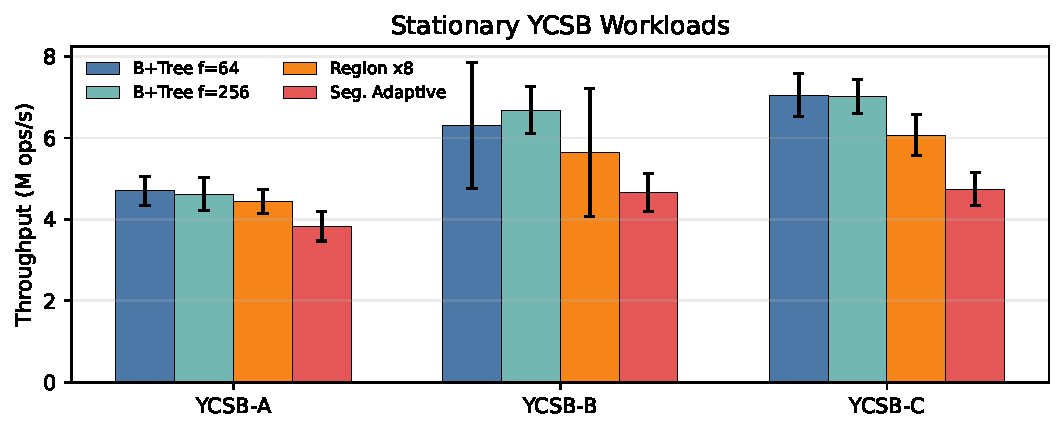
\includegraphics[width=\linewidth]{figures/fig_ycsb_throughput.pdf}
  \caption{Five-trial YCSB throughput.  Error bars show 95\% confidence
  intervals.  Segmented adaptation is consistently below static fanout 64.}
  \Description{Bar chart comparing throughput for static and adaptive indexes
  on YCSB workloads A, B, and C.}
  \label{fig:ycsb}
\end{figure}

\begin{table}[t]
\centering
\caption{Five-trial YCSB throughput summary.}
\label{tab:ycsb}
\begin{tabular}{lrrrr}
\toprule
Workload & Static f64 & Best static & Seg. adaptive & Seg./f64 \\
\midrule
YCSB-A & 4.70M & 4.70M & 3.83M & 0.81 \\
YCSB-B & 6.30M & 6.68M & 4.65M & 0.74 \\
YCSB-C & 7.04M & 7.04M & 4.74M & 0.67 \\
\bottomrule
\end{tabular}
\end{table}

\subsection{Shifting Hot Regions}

The shifting workload gives adaptation a fairer opportunity because locality
changes over time.  Figure~\ref{fig:shifting} plots selected per-phase
results.  The oracle with hot fanout 32 reaches \(1.08\times\) aggregate
throughput over static fanout 64, confirming that fanout adaptation has
headroom.  However, segmented adaptation reaches only \(0.92\times\).  Static
regional fanout 256 reaches \(1.13\times\), showing that coarse static
partitioning can be more effective than online adaptation.

\begin{figure}[t]
  \centering
  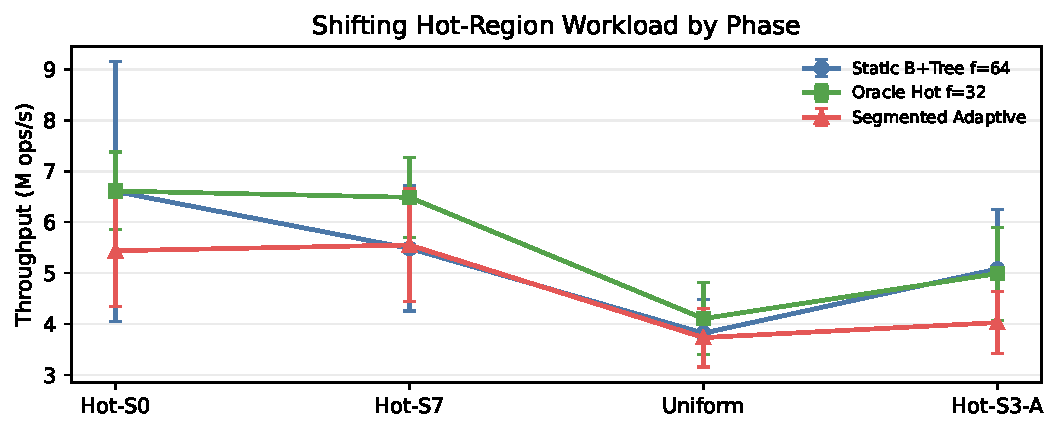
\includegraphics[width=\linewidth]{figures/fig_shifting_phases.pdf}
  \caption{Shifting hot-region throughput by phase.  The oracle shows
  measurable headroom, but online segmented adaptation does not capture it.}
  \Description{Line chart of throughput across hot-region phases for static,
  oracle, and segmented adaptive indexes.}
  \label{fig:shifting}
\end{figure}

\begin{table}[t]
\centering
\caption{Aggregate shifting workload throughput.}
\label{tab:shifting}
\begin{tabular}{lrr}
\toprule
Index & Throughput & vs f64 \\
\midrule
Static Region f256 & 5.53M & 1.13 \\
Oracle Hot f32 & 5.29M & 1.08 \\
Static B+Tree f256 & 5.24M & 1.07 \\
Static B+Tree f64 & 4.86M & 1.00 \\
Segmented Adaptive & 4.49M & 0.92 \\
\bottomrule
\end{tabular}
\end{table}

\subsection{Wikipedia Pageview Trace}

Table~\ref{tab:wiki} shows the real-trace result.  Static fanout 256 and
fanout 64 are nearly identical: 10.42M and 10.39M operations/s.  Thus the
workload has almost no fanout-selection headroom at this scale.  Segmented
adaptation reaches 8.40M operations/s, or \(0.81\times\) of static fanout 64.
The trace is skewed, but the hot working set is small enough that static
fanout choice is not the limiting factor.

\begin{table}[t]
\centering
\caption{Wikipedia pageview trace throughput.}
\label{tab:wiki}
\begin{tabular}{lrr}
\toprule
Index & Throughput & vs f64 \\
\midrule
Static B+Tree f256 & 10.42M & 1.00 \\
Static B+Tree f64 & 10.39M & 1.00 \\
Static Region f32 & 10.19M & 0.98 \\
Static Region x8 & 9.88M & 0.95 \\
Segmented No Adapt & 8.79M & 0.85 \\
Segmented Adaptive & 8.40M & 0.81 \\
\bottomrule
\end{tabular}
\end{table}

\subsection{Clean Overhead Ablation}

Figure~\ref{fig:overhead} and Table~\ref{tab:overhead} isolate the access-path
costs.  The values are intentionally not monotone in every row: cache
placement, routing, and run-to-run noise can make one row faster than the
previous row.  The robust pattern is that the full adaptive path is below
static on Zipf-A and Zipf-B and below the best static regional rows.  In
Zipf-A, the records-only row reaches 4.90M operations/s, the monitor-plus-
records row reaches 4.60M operations/s, and full adaptation reaches 3.91M
operations/s.

\begin{figure}[t]
  \centering
  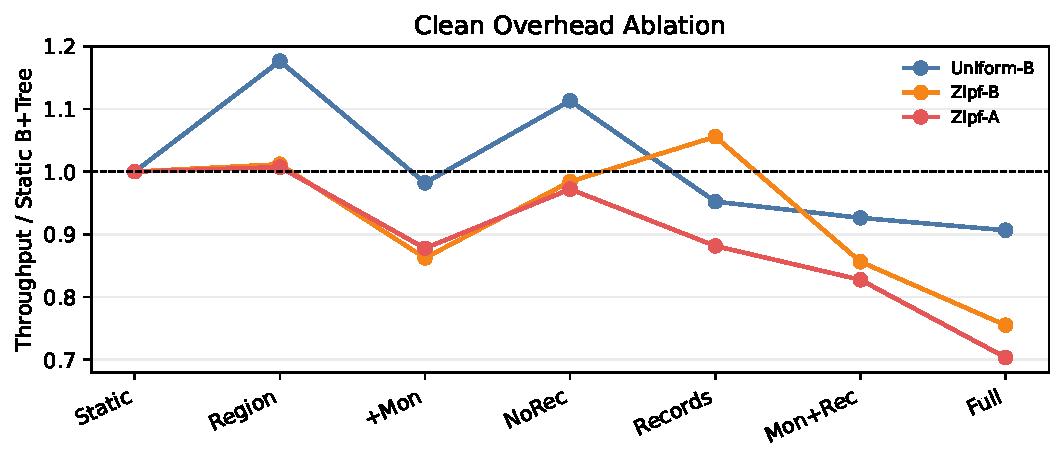
\includegraphics[width=\linewidth]{figures/fig_overhead_ablation.pdf}
  \caption{Clean overhead ablation normalized to Static B+Tree.  The full
  adaptive path includes routing, records, monitoring, policy checks, and
  rebuild decisions.}
  \Description{Line chart of normalized throughput across the seven ablation
  configurations.}
  \label{fig:overhead}
\end{figure}

\begin{table*}[t]
\centering
\caption{Clean overhead ablation.  Ratios are relative to the previous
conceptual baseline named in each column.}
\label{tab:overhead}
\resizebox{\textwidth}{!}{%
\begin{tabular}{lrrrrrrr}
\toprule
Workload & Region/Static & Monitor/Region & NoRec/Region & Rec/NoRec &
MonRec/Rec & Full/MonRec & Full throughput \\
\midrule
Uniform-B & 1.18 & 0.83 & 0.95 & 0.86 & 0.97 & 0.98 & 4.79M \(\pm\) 0.41M \\
Zipf-A & 1.01 & 0.87 & 0.97 & 0.91 & 0.94 & 0.85 & 3.91M \(\pm\) 0.30M \\
Zipf-B & 1.01 & 0.85 & 0.97 & 1.07 & 0.81 & 0.88 & 5.68M \(\pm\) 0.42M \\
\bottomrule
\end{tabular}}
\end{table*}

\subsection{Concurrent Lookup Scalability}

The original prototype was single-threaded.  To test whether the baseline can
serve as a credible systems artifact, we added optimistic lock coupling to the
B+ tree.  Each node stores an atomic version word; readers validate versions
before and after traversal, while writers acquire per-node version locks.  The
thread benchmark preloads one million keys and executes ten million operations
with 95\% reads and 5\% updates.  Figure~\ref{fig:threads} and
Table~\ref{tab:threads} show that the baseline scales to the 16 hardware
threads of our i5-12500H and flattens under oversubscription at 32 worker
threads.  This result does not reverse the adaptive-index conclusion, but it
removes a major systems concern: the static baseline is not protected by a
single global lock.

\begin{figure}[t]
  \centering
  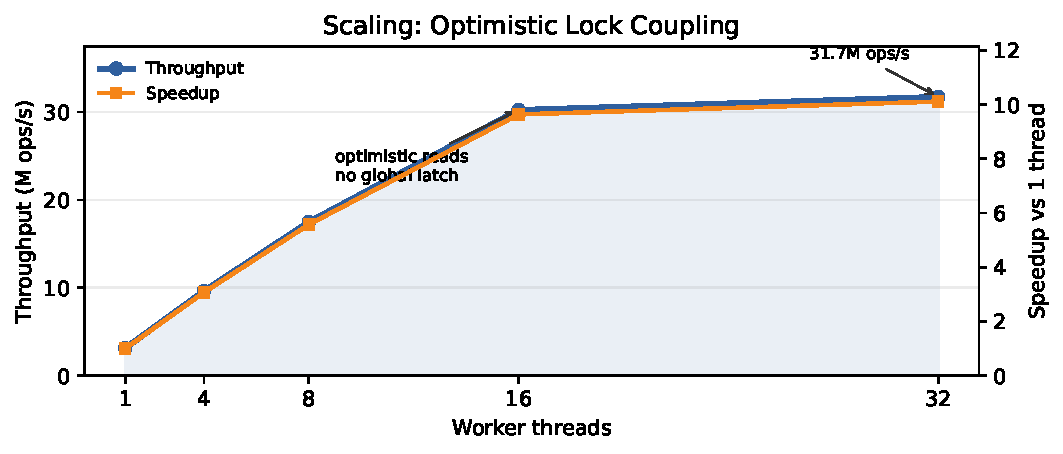
\includegraphics[width=\linewidth]{figures/fig_thread_scalability.pdf}
  \caption{Optimistic lock coupling scalability on a one-million-key tree and
  ten-million-operation workload.}
  \Description{Line chart showing throughput and speedup as worker threads
  increase from 1 to 32.}
  \label{fig:threads}
\end{figure}

\begin{table}[t]
\centering
\caption{Thread-scalability benchmark, 95\% reads and 5\% updates.}
\label{tab:threads}
\begin{tabular}{rrr}
\toprule
Threads & Throughput & Speedup \\
\midrule
1 & 3.14M & 1.00 \\
4 & 9.63M & 3.07 \\
8 & 17.48M & 5.57 \\
16 & 30.21M & 9.64 \\
32 & 31.70M & 10.11 \\
\bottomrule
\end{tabular}
\end{table}

\subsection{Rapidly Shifting Hotspots}

We also add a sliding-hotspot benchmark.  The workload contains one million
keys and five one-million-operation windows.  In each window, 80\% of accesses
target a Zipfian hot region covering 20\% of the key space; the hot region
moves to a disjoint range in the next window.  This benchmark is intentionally
hostile to stale predictors.  Figure~\ref{fig:dynamic} and
Table~\ref{tab:dynamic} show that the adaptive tree does not catch up: the
cost gate evaluates many adaptation opportunities but performs no rebuilds,
and the full segmented adaptive path reaches only \(0.63\times\) the static
B+ tree throughput.  This strengthens the paper's negative result because the
workload gives adaptation fresh skew but too little safe headroom to exploit.

\begin{figure}[t]
  \centering
  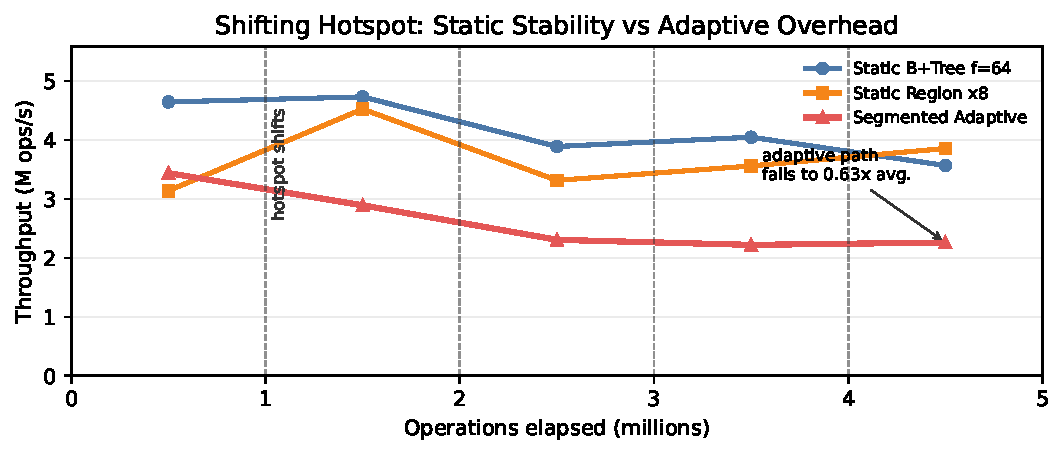
\includegraphics[width=\linewidth]{figures/fig_dynamic_hotspot.pdf}
  \caption{Sliding-hotspot throughput by one-million-operation window.  The
  adaptive tree tracks accesses but remains below static fanout 64.}
  \Description{Line chart comparing static, static regional, and segmented
  adaptive throughput over five shifting-hotspot windows.}
  \label{fig:dynamic}
\end{figure}

\begin{table}[t]
\centering
\caption{Sliding-hotspot aggregate throughput.}
\label{tab:dynamic}
\begin{tabular}{lrr}
\toprule
Index & Throughput & vs Static f64 \\
\midrule
Static B+Tree f64 & 4.18M & 1.00 \\
Static Region x8 & 3.68M & 0.88 \\
Segmented Adaptive & 2.62M & 0.63 \\
\bottomrule
\end{tabular}
\end{table}

\subsection{Memory Reclamation and Reader Safety}

Optimistic reads raise a standard systems question: if readers traverse
without latches, when is it safe to reclaim old nodes?  The implementation
used for the concurrency benchmark avoids unsafe reclamation in two ways.
First, the benchmark preloads the tree and then executes lookups and in-place
updates; updates overwrite existing values and do not delete nodes.  Second,
structural splits are publication-only: a split allocates a new node and links
it into the tree, while the old node remains valid.  The tree is destroyed
only after all worker threads have joined.  Thus a reader that validates an
old version can safely retry without dereferencing freed memory.

Segment rebuilds for adaptive fanout are more subtle.  In the current
experiments, segmented rebuilds are evaluated in the single-threaded adaptive
benchmarks, not concurrently with the multi-threaded lookup benchmark.  A
fully concurrent adaptive tree should retire replaced segment roots using
epoch-based reclamation: each worker publishes its active epoch before
traversal, writers place old roots on a retire list, and a retired tree is
freed only after all active readers have advanced beyond the retire epoch.
This is an engineering constraint rather than a change to the break-even
model; epoch management would add another small term to the online overhead
\(\mu\).

\section{Theoretical Analysis}

We now formalize the cost argument.  The theory has two roles.  First, it
shows that restructuring itself can be amortized if the algorithm waits for
enough evidence.  Second, it shows why that amortization is insufficient when
per-operation monitoring and metadata costs exceed the fanout benefit.

\subsection{Amortized Restructuring}

Let a segment maintain a nonnegative potential \(\Phi_t\).  Each operation
adds at most a constant \(\gamma\) units of potential.  A rebuild of cost
\(R_t\) is allowed only when \(\Phi_t \ge R_t\), and when it rebuilds the
algorithm spends \(R_t\) units of potential.

\begin{theorem}
If the rebuild rule above is enforced, restructuring has \(O(1)\) amortized
cost per operation.
\end{theorem}

\begin{proof}
Let \(a_t\) be the actual restructuring cost at operation \(t\), and define
the amortized cost
\[
  \hat{a}_t = a_t + \Phi_{t+1}-\Phi_t .
\]
If no rebuild occurs, \(a_t=0\) and \(\Phi_{t+1}-\Phi_t\le\gamma\), so
\(\hat{a}_t\le\gamma\).  If a rebuild occurs, then \(a_t=R_t\) and the
potential decreases by at least \(R_t\), except for the current operation's
new credit:
\[
  \Phi_{t+1}-\Phi_t \le \gamma - R_t .
\]
Thus \(\hat{a}_t \le R_t+\gamma-R_t=\gamma\).  Summing over \(T\)
operations telescopes the potential terms, giving total restructuring cost
\(O(T)\), or \(O(1)\) amortized cost per operation.
\end{proof}

\subsection{Competitive Bound}

Let \(\mathcal{F}=\{2,4,16,256,\ldots,2^{2^j}\le n\}\) be a geometric
fanout ladder.  Then \(|\mathcal{F}|=O(\log\log n)\).  Suppose that for every
oracle fanout \(f^\star\), some \(f\in\mathcal{F}\) has cost within a constant
factor \(\alpha\) of \(f^\star\).  An online policy that may test all fanouts
in \(\mathcal{F}\) during a stable phase pays at most \(O(|\mathcal{F}|)\)
times the best ladder fanout cost, plus online overhead.

\begin{theorem}
Under the regularity condition above, and assuming rebuilds are amortized by
the potential rule, the online adaptive tree has
\[
  \mathrm{Cost}(\mathrm{A})
  \le O(\log\log n)\cdot \mathrm{Cost}(\mathrm{OPT}) + O(T\mu),
\]
where \(T\) is the number of operations and
\(\mu=m+r+p\) is monitoring, records, and policy overhead per operation.
\end{theorem}

\begin{proof}
Let \(k=|\mathcal{F}|=O(\log\log n)\).  In a phase, the online policy can
spend at most one testing epoch on each of the \(k\) fanouts before using the
best observed candidate.  The phase cost is therefore bounded by
\[
  O(k)\cdot T_P \min_{f\in\mathcal{F}} c_f(n_P) + O(T_P\mu),
\]
where the rebuild term is absorbed by the \(O(T_P)\) amortized bound from the
previous theorem.  By regularity, the best ladder fanout is within a constant
factor of the oracle fanout for that phase.  Summing over phases gives the
claimed bound.
\end{proof}

The additive \(O(T\mu)\) term is exactly the problem measured in this paper.
The competitive bound is meaningful only when \(\mu\) is small relative to the
oracle's operation cost.  In our in-memory workloads, \(\mu\) is not small.

\subsection{Break-Even Condition}

The measurements can be explained by a simple condition.  Consider a phase of
\(T\) operations in a segment with incumbent fanout \(F_0\) and candidate
fanout \(F_1\).  Let
\[
  \Delta = C(F_0,N_s)-C(F_1,N_s)
\]
be the per-operation fanout benefit.  Let \(m\), \(\rho\), and \(d\) be the
per-operation costs of monitoring, records metadata, and policy evaluation,
and let \(R\) be the one-time rebuild cost.  Adaptation improves total time
only if
\[
  T(\Delta - m - \rho - d) > R.
\]
Equivalently, if \(\Delta \le m+\rho+d\), no phase length can make online
adaptation profitable.

Figure~\ref{fig:benefit} compares measured headroom with measured penalty.  On
YCSB-A, the adaptive penalty is approximately 0.047 \us/op; on YCSB-B and
YCSB-C it is roughly 0.060 and 0.055 \us/op.  On the shifting workload, the
oracle benefit is about 0.011--0.013 \us/op, while adaptation costs about
0.014--0.025 \us/op depending on the comparison.  On the Wikipedia trace, the
static fanout-selection benefit is only about 0.0003 \us/op, while the adaptive
penalty is about 0.023 \us/op.

\begin{figure}[t]
  \centering
  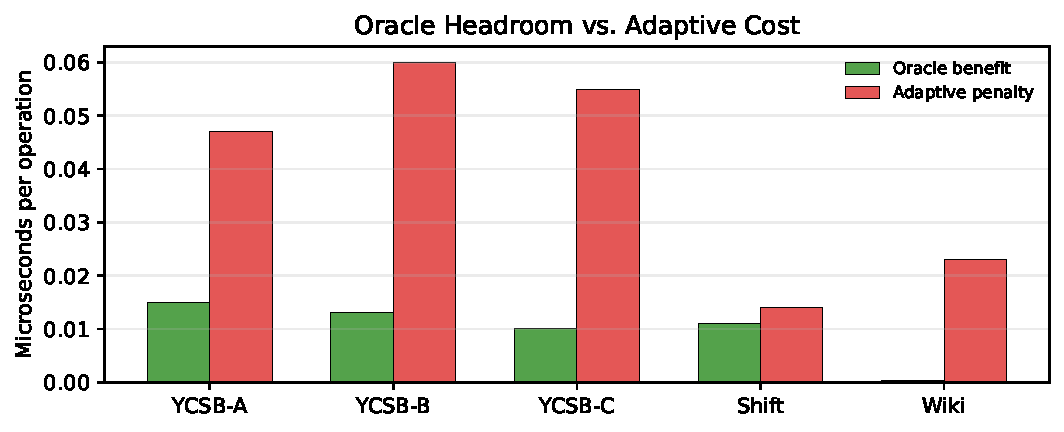
\includegraphics[width=\linewidth]{figures/fig_benefit_vs_penalty.pdf}
  \caption{Measured oracle headroom versus adaptive penalty.  In every tested
  case, the online cost is comparable to or larger than the available benefit.}
  \Description{Bar chart comparing oracle benefit and adaptive penalty in
  microseconds per operation.}
  \label{fig:benefit}
\end{figure}

This model does not say that adaptation is impossible.  It says adaptation must
be judged at the same time scale as the operation it improves.  For in-memory
B-trees with sub-microsecond lookups, software monitoring and rebuild decisions
are expensive.  For disk-resident trees, remote memory, or very long stable
phases, the benefit term \(\Delta\) may become large enough to dominate.

\section{Discussion}

\subsection{Why This Negative Result Matters}

The adaptive variants fail despite multiple policies, cost-aware rebuild
gates, and workloads designed to expose skew.  The failure is therefore not
best understood as a single bad policy.  It is a cost/benefit mismatch.  The
oracle rows show that choosing a better fanout can help.  The overhead rows
show that observing and acting on that opportunity can cost more than the
opportunity itself.

\subsection{When Adaptation Might Work}

The break-even condition suggests several scenarios where online fanout
adaptation could still be viable.  First, disk-resident or remote-memory trees
may have much larger fanout benefit because a height reduction can avoid
expensive I/O.  Second, workloads with very long stable phases can amortize
rebuild cost.  Third, hardware-assisted monitoring might reduce \(m\), although
it would not remove metadata and rebuild cost.  Fourth, coarser adaptation at
the granularity of entire indexes or partitions may be more practical than
per-node or per-small-segment adaptation.

\subsection{Practical Recommendation}

For in-memory indexes at this scale, static tuning and coarse regional layout
are safer than online fine-grained fanout adaptation.  Practitioners should
profile a representative workload and choose a static fanout or a small set of
static regional fanouts.  Researchers proposing adaptive index structures
should include oracle baselines and component ablations; otherwise it is
difficult to tell whether the design captures real headroom or merely shifts
costs.

\section{Related Work}

B-trees and B+ trees are foundational ordered indexes
\cite{bayer1972organization,comer1979ubiquitous,graefe2011modern}.  Prior
cache-conscious designs optimize node layout, prefetching, and memory access
patterns \cite{rao1999cache,rao2000making,chen2001fractal}.  Cache-oblivious
trees study asymptotic transfer bounds without explicit cache parameters
\cite{bender2000cache}.  Our work differs by testing online fanout changes and
measuring the cost of making the decision at runtime.

Adaptive and workload-aware indexing has a long history.  Splay trees adjust
to access patterns through rotations \cite{sleator1985self}.  Database
cracking and adaptive merging progressively refine physical organization based
on queries \cite{idreos2007database,idreos2011adaptive}.  ART changes node
representation based on local key density \cite{leis2013adaptive}.  Learned
indexes and learned variants adapt model structure or error bounds to data
distributions \cite{kraska2018case,ding2020alex,galakatos2019fiting}.  These
systems motivate our question, but they do not isolate online fanout adaptation
costs in B-trees.

Self-tuning database systems select indexes, views, or configurations at much
coarser time scales \cite{chaudhuri1998autoadmin,weikum2002selftuning,
pavlo2017selfdriving}.  Our result is consistent with that design lesson:
adaptation is easier to justify when the cost is amortized over many
operations.  Fine-grained adaptation on a sub-microsecond access path is a much
harsher setting.

\section{Conclusion}

We implemented adaptive B-tree fanout selection and expected skewed workloads
to benefit.  The data instead supports a diagnostic negative result.  Static
fanout choices and oracle phase-aware fanouts have measurable headroom, but the
online path pays monitoring, metadata, policy, and rebuild costs that exceed
the benefit on our in-memory workloads.

The resulting lesson is constructive.  Adaptive index papers should measure
both oracle headroom and adaptation overhead.  If the oracle cannot beat the
baseline, no online method can win; if the oracle wins only slightly, software
adaptation must be nearly free.  For the workloads tested here, fine-grained
online fanout adaptation is not yet a practical replacement for static tuning
or coarse regional indexing.

\begin{acks}
We thank the database systems community for emphasizing reproducibility,
negative results, and careful baselines.  Funding and acknowledgments should be
added here before submission.
\end{acks}

\bibliographystyle{ACM-Reference-Format}
\bibliography{references}

\end{document}
